\documentclass[svgnames]{article}
\usepackage{tikz,amsmath}

\usepackage{graphicx}
\pagestyle{empty}
\begin{document}

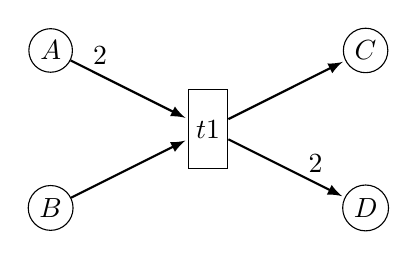
\begin{tikzpicture}[scale=1]
%%% Toy PN
\node[shape=circle, draw, inner sep=2pt]  (A) at (0,2) {$A$};
\node[shape=circle, draw, inner sep=2pt]  (B) at (0,0) {$B$};
\node[shape=circle, draw, inner sep=2pt]  (C) at (4,2) {$C$};
\node[shape=circle, draw, inner sep=2pt]  (D) at (4,0) {$D$};
\node[shape=rectangle, draw,minimum height=1cm,minimum width=0.5cm,inner sep=2pt]  (t1) at (2,1) {$t1$};

\draw[-latex,thick,shorten >=1pt](A)--(t1)node[near start,above] {$2$};
\draw[-latex,thick,shorten >=1pt](B)--(t1);
\draw[-latex,thick,shorten >=1pt](t1)--(C);
\draw[-latex,thick,shorten >=1pt](t1)--(D)node[near end,above] {$2$};

%\draw[-|,thick,shorten >=1pt](A)..controls(2.7,2.3) and (2.7,1.7)..(A);
%\draw[->,thick](B)--(C);
%\draw[->,thick](C)--(A);

\end{tikzpicture}

\end{document}
